\chapter{DBMS}
% ! È già presente nell'introduzione questa definizione
\begin{definizione}[\textbf{DBMS}]
      Un \textbf{DBMS} (DataBase Management System) è un sistema software in grado
      di gestire collezioni di dati che siano:
      \begin{itemize}
            \item \textbf{Grandi}: di dimensioni molto maggiori rispetto alla memoria
                  centrale dei sistemi di calcolo utilizzati.
            \item \textbf{Persistenti}: i dati devono essere memorizzati su un
                  supporto di memorizzazione non volatile. Il periodo di vita dei
                  dati è indipendente dalle singole esecuzioni dei programmi che li
                  utilizzano.
            \item \textbf{Condivisi}: i dati devono essere accessibili da più utenti
                  contemporaneamente e anche da applicazioni diverse.
            \item \textbf{Affidabili}: devono essere resistenti a guasti.
      \end{itemize}
\end{definizione}
I DBMS sono solitamente posizionati tra la base di dati fisica e le applicazioni
che la utilizzano. Questo permette di separare la gestione dei dati dalla
gestione delle applicazioni, permettendo di modificare le applicazioni senza
modificare i dati e viceversa.

Le principali caratteristiche di un DBMS Centralizzato sono:
\begin{itemize}
      \item Un unico schema logico, ovvero un'unica semantica.
      \item Un'unica base di dati, ovvero un unico insieme di record interrogati
            ed aggiornati da tutti gli utenti.
      \item Nessuna forma di eterogeneità concettuale.
      \item Un unico schema fisico, ovvero un'unica rappresentazione fisica dei
            dati.
      \item Nessuna distribuzione e nessuna eterogeneità fisica.
      \item Un unico linguaggio di interrogazione, quindi un'unica modalità di
            accesso e selezione dei dati di interesse.
      \item Un unico sistema di gestione, quindi un'unica modalità di accesso,
            aggiornamento e gestione delle transazioni.
      \item Un'unica modalità di ripristino a fronte di guasti.
      \item Un unico amministratore dei dati e quindi nessuna autonomia gestionale.
\end{itemize}

Visto che i DBMS sono \textbf{grandi} e \textbf{persistenti}, spesso più grandi
della memoria centrale, allora le principali azioni che essi devono compiere
riguardano quindi la \textbf{memorizzazione fisica efficiente} delle strutture
dati nella memoria secondaria e la \textbf{scelta efficiente delle pagine} da
trasferire nel buffer della memoria centrale.

Una base di dati è una \textbf{risorsa integrata e condivisa} fra le varie
applicazioni, questo rende necessario introdurre dei meccanismi di
\textbf{autorizzazione e di controllo della concorrenza} per controllare gli
accessi. In un mondo ideale, le \textbf{transazioni} sono \textbf{corrette} se
sono \textbf{seriali}, ma questo penalizzerebbe di molto l'efficienza del sistema e
quindi il \textbf{controllo della concorrenza} permette un ragionevole compromesso.
% ! Fino a qui è già presente nell'introduzione

Quando gli utenti eseguono le \textbf{query} sulle basi di dati, lo fanno avendo
a disposizione lo schema logico. Questo schema però non rappresenta come sono
realmente memorizzati i dati, inoltre, le rappresentazioni logiche sono poco
efficienti in memoria secondaria. Per questo motivo, i DBMS devono
\textbf{tradurre} le query in modo da ridurre al minimo il numero di accessi
alla memoria secondaria, quindi si effettuerà un'\textbf{ottimizzazione delle query}.

Un modo per gestire l'\textbf{affidabilità} delle basi di dati è quello di utilizzare
\textbf{transizioni atomiche} e \textbf{definitive}, ovvero operazioni che
vengono eseguite completamente o non vengono eseguite affatto. Questo permette
di mantenere la consistenza dei dati anche in caso di guasti.

L'architettura dietro ad un DBMS centralizzato è raffigurata nella figura \ref{fig:DBMS_architecture}
\begin{figure}[!ht]
      \centering
      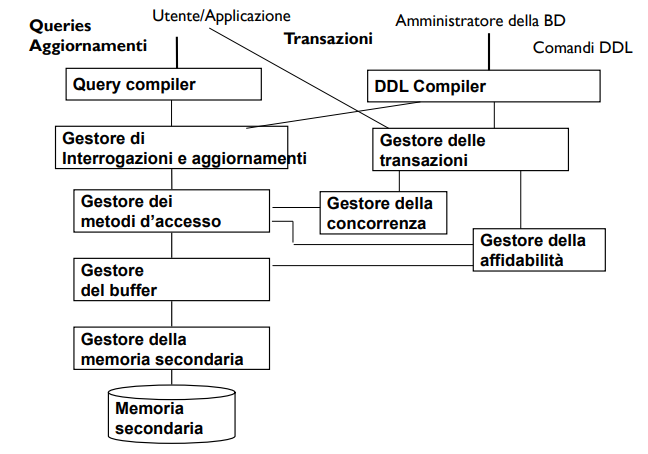
\includegraphics[width=0.7\textwidth]{./img/DBMS/Architettura.png}
      \caption{Architettura di un DBMS}
      \label{fig:DBMS_architecture}
\end{figure}
\section{Gestione degli accessi e delle interrogazioni}
La gestione degli accessi e delle interrogazioni inizia con la struttura del database
espressa Database administrator mediante i comandi DDL che vengono interpretati
dal DDL compiler e nel DBMS viene costruita la struttura dello schema.

A questo punto, il \textbf{Query compiler} si occupa di compilare le queries e le
passa al \textbf{gestore delle interrogazioni} che le ottimizza e le frammenta in
comandi elementari di accesso, che invia al \textbf{gestore dei metodi di accesso},
che li trasforma in comandi di accesso a pagine (quindi in comandi per l'accesso
alla struttura in memoria), che invia al \textbf{gestore del buffer}, il quale è
responsabile della ottimizzazione. In seguito, invia i comandi al \textbf{gestore
      della memoria secondaria}, che si occupa tradurre i comandi in accessi alle
pagine sul disco.
\section{Gestione delle transazioni}
Il \textbf{gestore delle transazioni} si occupa di eseguire le transazioni e
garantire, interagendo col \textbf{gestore dell'affidabilità} e il \textbf{gestore
      della concorrenza} (scheduler), che le transazioni rispettino le proprietà
di atomicità, consistenza, isolamento e durabilità (ACID).
\section{Ottimizzazione delle interrogazioni}
La fase di ottimizzazione delle interrogazioni è suddivisa in diversi passaggi:
\begin{enumerate}
      \item Verificare che la query sia sintatticamente corretta. Per fare ciò,
            si utilizza il \textbf{Data Catalog}, che contiene le informazioni
            riguardanti la struttura dello schema.
            Questa operazione traduce la query in algebra relazionale e costruisce
            successivamente un query tree.
      \item Si trasforma un query tree in un query plan logico che viene ottimizzato
            per ridurre il suo costo di esecuzione. Per l'ottimizzazione si
            utilizza un altro database particolare è \textbf{Statistics}
            contenente statistiche sulla storia di esecuzioni precedenti delle
            interrogazioni.
      \item Si trasformano le espressioni scritte in algebra relazionale in
            espressioni che possono essere eseguite in modo efficiente. (si
            ottimizza l'espressione di algebra relazionale)
      \item Si trasforma il query plan logico in un query plan fisico, ovvero
            si mappano le operazioni dell'algebra relazionale sulle loro
            implementazioni per l'accesso alle strutture dati in memoria e si eseguono.
\end{enumerate}
\begin{nota}
      In generale l'ottimizzazione del query plan avviene anticipando il prima possibile
      le selezioni e posticipando il più possibile le join in modo da ridurre il più
      possibile la dimensione delle tabelle che sono da unire.
\end{nota}
\begin{definizione}[\textbf{Query Tree}]
      La query viene rappresentata come un albero nel quale:
      \begin{itemize}
            \item Le foglie corrispondono alle strutture dati logiche (tabelle).
            \item I nodi intermedi rappresentano operazioni algebriche:
                  \begin{itemize}
                        \item Selezione
                        \item Proiezione
                        \item Join
                        \item Prodotto cartesiano
                        \item Operazioni insiemistiche
                  \end{itemize}
      \end{itemize}
\end{definizione}
Chiaramente queste trasformazioni vengono eseguire mediante una strategia che
usa proprietà algebriche e una stima dei costi delle operazioni fondamentali per
i diversi metodi di accesso. In generale il problema di ottimizzazione delle
query è esponenziale, ma si utilizzano delle approssimazioni ragionevoli basate
su euristiche.
\begin{figure}[!ht]
      \centering
      \includegraphics[width=0.7\textwidth]{./img/DBMS/Ottimizzazione_query.png}
      \caption{Ottimizzazione delle interrogazioni}
      \label{fig:Query_Optimization}
\end{figure}
% TODO: aggiungere immagine su un esempio di ottimizzazione di una query SQL
\section{Gestione delle transazioni}
Le transazioni sono degli insiemi di istruzioni di lettura e scrittura sulla base
di dati che godono di alcune proprietà che permettono la loro corretta esecuzione
in \textbf{ambienti concorrenti} e \textbf{non affidabili}.

Generalmente vengono identificate da un inizio begin - transaction e una fine
end - transaction e al cui interno deve essere eseguito una e una sola
volta uno dei seguenti comandi:
\begin{itemize}
      \item \textbf{commit work} per terminare correttamente
      \item \textbf{rollback work} per abortire la transazione e ripristinare lo
            stato iniziale della transazione.
\end{itemize}
Un \textbf{sistema transazionale} (OLTP) è in grado di definire ed eseguire
transazioni per un certo numero di applicazioni concorrenti.

Le transazioni godono delle proprietà \textbf{ACID}:
\begin{itemize}
      \item \textbf{Atomicità}: una transazione è un'unità indivisibile di
            esecuzione che deve essere eseguita completamente o non deve essere
            eseguita affatto.
      \item \textbf{Consistenza}: una transazione deve portare il database da uno
            stato consistente ad un altro stato consistente. Durante l'esecuzione
            di una transazione si possono avere mancanze di consistenze, l'importante
            è che al suo termine la consistenza deve essere mantenuta.
      \item \textbf{Isolamento}: le transazioni devono essere eseguite in modo
            indipendente l'una dall'altra.
      \item \textbf{Durabilità}: una transazione che ha terminato con successo
            deve essere persistente anche in caso di guasti.
\end{itemize}
Se queste proprietà non sono rispettate si possono verificare delle anomalie,
come:
\begin{itemize}
      \item \textbf{Loss updates}: due transazioni leggono lo stesso
            dato, lo modificano e lo scrivono, ma solo una delle due modifiche
            viene mantenuta.
      \item \textbf{Dirty reads}: una transazione legge un dato che è stato
            modificato da un'altra transazione e non ancora committato.
      \item \textbf{Non-repeatable reads}: una transazione legge due
            volte lo stesso dato e ottiene due valori diversi.
      \item \textbf{Phantom reads}: una transazione legge due volte lo stesso
            insieme di dati e ottiene due insiemi diversi.
\end{itemize}
\subsection{Gestione della concorrenza}
La gestione della concorrenza è necessaria per garantire l'isolamento delle
transazioni. Questo è necessario perché le transazioni possono essere eseguite
in modo concorrente e quindi possono accedere contemporaneamente agli stessi
dati.
\begin{definizione}[\textbf{Schedule}]
      Una sequenza di esecuzione di un insieme di transizioni è detta \textbf{schedule}.
\end{definizione}
\begin{definizione}
      Uno \textbf{schedule} si dice \textbf{seriale} se una transazione è eseguita
      per intero prima che un'altra inizi.
\end{definizione}
Si sfrutta quindi la proprietà di isolamento facendo in modo che ogni
transazione esegua come se non ci fosse concorrenza.

Si ha quindi che uno schedule è serializzabile se l'esito della sua esecuzione è
lo stesso che si avrebbe con una qualsiasi sequenza seriale delle transazioni
contenute.

Si hanno quindi diversi algoritmi per il controllo della concorrenza secondo
varie tipologie:
\begin{itemize}
      \item \textbf{Controllo basato su conflict equivalente}
      \item \textbf{Controllo di concorrenza basato su locks} (protocollo 2PL o two
            phase locking, shared locks e gestione dei deadlock). Il protocollo
            2PL è usato nei DBMS dove per costruzione si hanno schedule
            serializzabili usando i lock per bloccare l'accesso alla risorse da
            parte di una transazione fino a che una risorsa non sia rilasciata.
            Si hanno quindi i concetti di lock e unlock che garantiscono l'uso
            esclusivo di una risorsa e l'autorizzazione esclusiva dell'uso di una
            risorsa viene dato dal gestore delle transazioni. I lock si possono
            richiedere su tabelle, database o porzioni di tabelle.
            Inoltre, in ogni transazione, tutte le richieste di lock precedono tutte
            le richieste di unlock. L'utilizzo dei lock è trasparente rispetto alle
            transazioni, infatti si avrà un TM (transaction manager) che gestirà
            l'accesso alla risorsa tenendo traccia delle risorse già impegnate e quelle
            libere. Inoltre, il TM aggiunge le richieste di lock e unlock alle
            transazioni in automatico per preservare il comportamento serializzabile.
      \item \textbf{controllo di concorrenza basato su timestamps}
\end{itemize}